\documentclass{beamer}
\usepackage[T1]{fontenc}
\usepackage[utf8]{inputenc}
\usepackage{listings}
\usepackage{caption}
\usepackage{amssymb}
\usepackage{upgreek}
\usepackage{mathtools}
\usepackage[backend=biber, style=alphabetic, language=british]{biblatex}
\usepackage{bookmark}
\usepackage{graphicx}
\graphicspath{ {./images/} }
\usepackage{tikz}
\usetikzlibrary{shapes.callouts,shadows, calc}

\AtEveryBibitem{%
  \clearfield{pages}%
  \clearfield{volume}%
  \clearfield{number}%
  \clearfield{url}%
  \clearfield{urldate}%
  \clearfield{isbn}%
}

\usepackage{color}
%colors for lean syntax
\definecolor{keywordcolor}{rgb}{0.7, 0.1, 0.1}   % red
\definecolor{tacticcolor}{rgb}{0.0, 0.1, 0.6}    % blue
\definecolor{commentcolor}{rgb}{0.4, 0.4, 0.4}   % grey
\definecolor{symbolcolor}{rgb}{0.0, 0.1, 0.6}    % blue
\definecolor{sortcolor}{rgb}{0.1, 0.5, 0.1}      % green
\definecolor{attributecolor}{rgb}{0.7, 0.1, 0.1} % red

% To display lean code
\def\lstlanguagefiles{lstlean.tex}
% set default language
\lstset{language=lean, extendedchars=true}

\usetheme[compress]{Berlin}
\usecolortheme{default}

\bibliography{thesis} 

\newcommand{\bA}{\mathbb{A}}
\newcommand{\bB}{\mathbb{B}}
\newcommand{\bC}{\mathbb{C}}
\newcommand{\bD}{\mathbb{D}}
\newcommand{\bE}{\mathbb{E}}
\newcommand{\bF}{\mathbb{F}}
\newcommand{\bG}{\mathbb{G}}
\newcommand{\bH}{\mathbb{H}}
\newcommand{\bI}{\mathbb{I}}
\newcommand{\bJ}{\mathbb{J}}
\newcommand{\bK}{\mathbb{K}}
\newcommand{\bL}{\mathbb{L}}
\newcommand{\bM}{\mathbb{M}}
\newcommand{\bN}{\mathbb{N}}
\newcommand{\bO}{\mathbb{O}}
\newcommand{\bP}{\mathbb{P}}
\newcommand{\bQ}{\mathbb{Q}}
\newcommand{\bR}{\mathbb{R}}
\newcommand{\bS}{\mathbb{S}}
\newcommand{\bT}{\mathbb{T}}
\newcommand{\bU}{\mathbb{U}}
\newcommand{\bV}{\mathbb{V}}
\newcommand{\bW}{\mathbb{W}}
\newcommand{\bX}{\mathbb{X}}
\newcommand{\bY}{\mathbb{Y}}
\newcommand{\bZ}{\mathbb{Z}}

\newcommand{\fA}{\mathcal{A}}
\newcommand{\fC}{\mathcal{C}}
\newcommand{\fL}{\mathcal{L}}
\newcommand{\fF}{\mathcal{F}}
\newcommand{\fR}{\mathcal{R}}
\newcommand{\fV}{\mathcal{V}}
\newcommand{\fM}{\mathcal{M}}
\newcommand{\fP}{\mathcal{P}}
\newcommand{\fD}{\mathcal{D}}
\newcommand{\fO}{\mathcal{O}}
\newcommand{\fX}{\mathcal{X}}

\newcommand{\pr}[2]{\text{pr}_{#1}(#2)} %projection
\newcommand{\compl}[1]{#1^{c}} %complement
\newcommand{\id}{\text{id}} %identity
\newcommand{\preim}[2]{#1^{-1}(#2)} %preimage
\newcommand{\interior}[1]{\text{int}(#1)} %interior
\newcommand{\closure}[1]{\overline{#1}} %closure
\newcommand{\boundary}{\partial} %boundary
\newcommand{\restrict}[2]{\ensuremath{\left.#1\right|_{#2}}} %restriction
\newcommand{\seqclosure}[1]{\text{scl}(#1)} %sequential closure
\newcommand{\oball}[2]{\text{B}_{#1}(#2)} %open ball
\newcommand{\closedCell}[2]{\closure{e}_{#2}^{#1}} %closed n-cell
\newcommand{\openCell}[2]{e_{#2}^{#1}} %open n-cell
\newcommand{\cellFrontier}[2]{\partial e_{#2}^{#1}} %edge n-cell
\newcommand{\closedCellf}[2]{\closure{f}_{#2}^{#1}} %closed n-cell
\newcommand{\openCellf}[2]{f_{#2}^{#1}} %open n-cell
\newcommand{\cellFrontierf}[2]{\partial f_{#2}^{#1}} %edge n-cell
\newcommand{\norm}[1]{\left\lVert#1\right\rVert} %norm
\newcommand{\maximum}[2]{\text{max}(#1, #2)} %maximum
\newcommand{\inv}[1]{#1^{-1}} %inverse function
\newcommand{\tanbun}[1]{T#1} %tangent bundle of a manifold
\newcommand{\tanspace}[2]{T_{#1}#2} %tangent bundle of a manifold
\newcommand{\vecfields}[1]{\mathfrak{X}(#1)}
\newcommand{\smoothfunc}[1]{C^\infty(#1)}
\newcommand{\pushfwd}[2]{#1_*#2}
\newcommand{\direcderiv}[1]{\text{D}_{#1}} %directional derivative
\newcommand{\derivat}[2]{\text{d}#1_{#2}} %derivative at a point
\newcommand{\tancone}[2]{T_{#1}(#2)} %tangent cone

\newcommand{\mathlib}{\texttt{Mathlib}\xspace}%mathlib

\captionsetup{labelformat=empty}

%Information to be included in the title page:
\title{Inward Pointing Vectors on Manifolds with Corners}
\author{Hannah Scholz}
\institute[MI]{Mathematical Institute of the University of Bonn}
\date{06.11.2026}

\setbeamertemplate{enumerate items}[default]

\begin{document}

\frame{\titlepage}

\section{Manifolds with Corners}

\begin{frame}{Model with Corners}
We will focus on real manifolds. 

Let $E$ be a normed space over $\bR$ and $H$ a topological space. 

\begin{block}{Definition: Model with Corners}
A \emph{model with corners} from $E$ to $H$ is a partial equivalence $I \colon H \to E$ such that 
\begin{enumerate}[(i)]
  \item the forward and backward map are continuous,
  \item then source is the entirety of $H$, and 
  \item the range is convex and has nonempty interior. 
\end{enumerate}
\end{block}
\alert{Example picture here (one for boundary one for corners one circle)}
\end{frame}

\begin{frame}{Topological Manifold with Corners}
%\small
\begin{block}{Definition: Topological Manifold with Corners}
  A topological space $M$ is a \emph{topological $n$-manifold} if
  \begin{enumerate}[(i)]
    %\setlength{\itemsep}{0pt}
    \item $M$ is Hausdorff.
    \item $M$ is second-countable, i.e.\ $M$ has a countable base.
    \item $M$ is locally $H$, i.e.\ for every point $p$ there is a neighbourhood of $p$ that is homeomorphic to an open set in $H$.
  \end{enumerate}
\end{block}
\begin{block}{Definition: Chart}
Let $M$ be a topological manifold with corners. 
Let $U$ be an open subset of $M$ and $\varphi \colon U \to H$ a homeomorphism onto an open subset of $H$. 
Then we call $(U, \varphi)$ a chart of $M$. 
\end{block}
\end{frame}

\begin{frame}{Boundary of a Topological Manifold}
\setbeamertemplate{enumerate items}[default]
\begin{block}{Definition: Boundary}
Let $M$ be a topological manifold with boundary. 
\begin{enumerate}[(i)]
  \item A point $p \in M$ is a \emph{boundary point} if it is in the domain of a \emph{boundary chart}, i.e.\ a chart $(U, \varphi)$ with $I(\varphi(p)) \in \boundary (I(H))$. 
  \item A point $p \in M$ is an \emph{interior point} if it is in the domain of an \emph{interior chart}, i.e.\ a chart $(U, \varphi)$ with $I(\varphi(U)) \cap \boundary (I(H)) = \varnothing$. 
\end{enumerate}
\end{block}
\begin{figure}
\begin{minipage}[b]{0.8\linewidth}
  \centering
  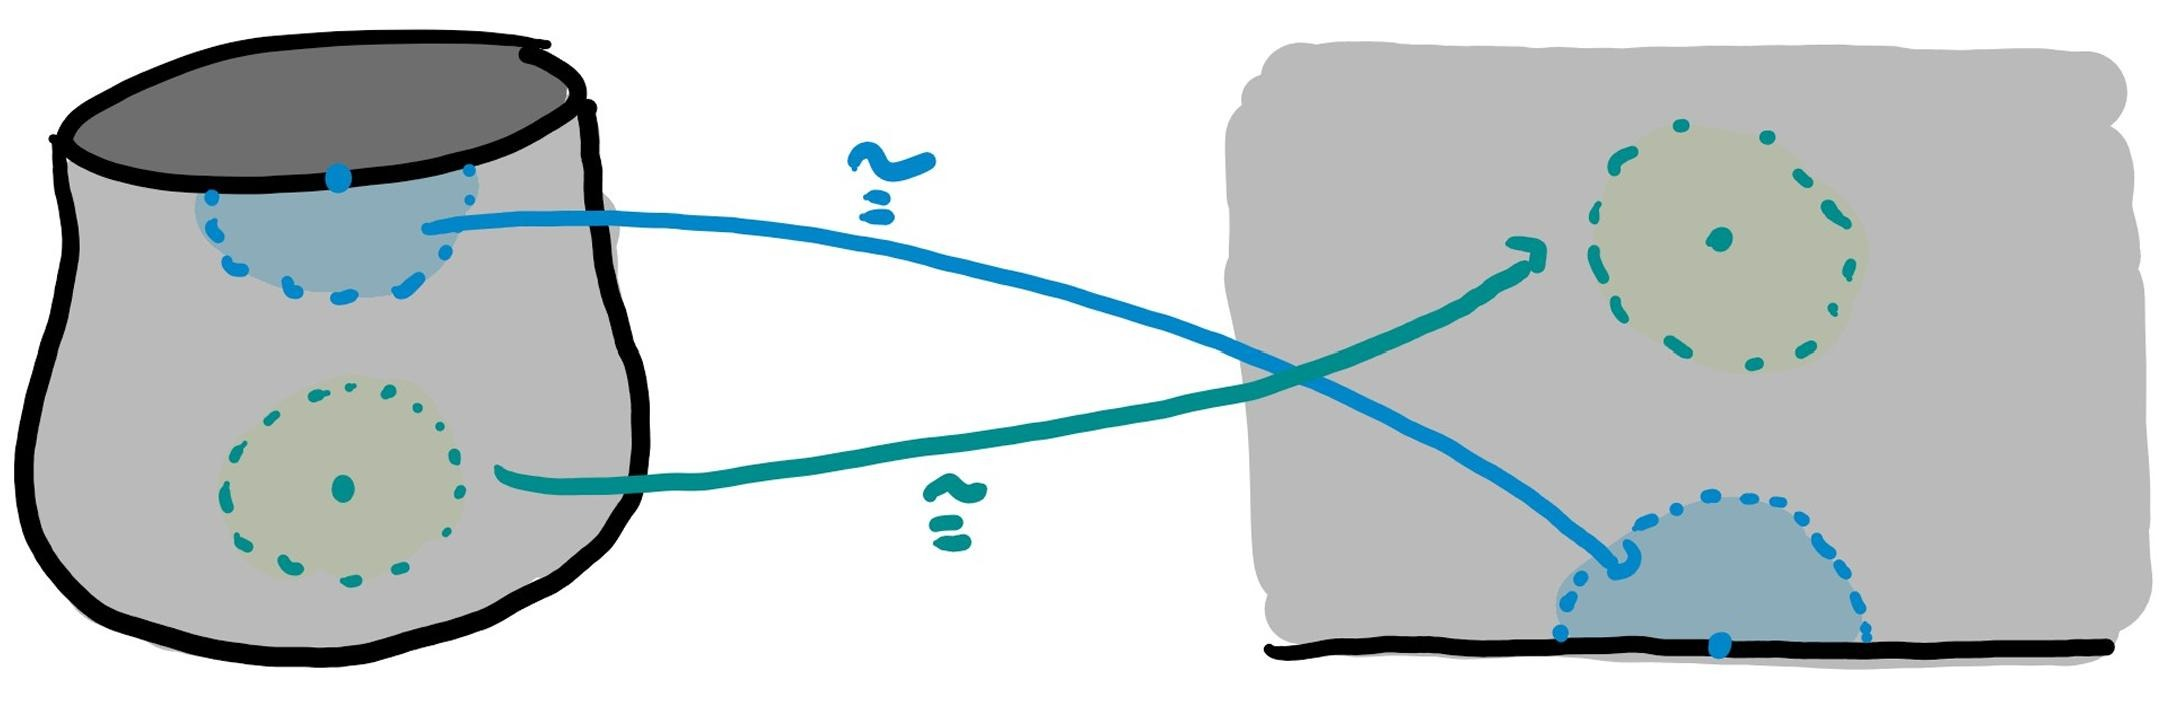
\includegraphics[width=\textwidth]{images/topologicalmanifold.png}
  %\caption{Topological manifold with a boundary and interior chart}
\end{minipage}
\end{figure}
\end{frame}

\begin{frame}{Smooth Manifold with Corners}
\begin{block}{Definition: Smooth Atlas}
Let $M$ be a topological manifold. 
Let $\fA$ be a collection of charts whose domains cover $M$.
$\fA$ is a smooth atlas for $M$ if any two charts $(\varphi, U)$ and $(\psi, V)$ are \emph{smoothly compatible}, i.e.\ either $U \cap V$ is empty or $I \circ\psi \circ \inv{\varphi} \circ \inv{I} \colon I(\varphi(U \cap V)) \to \psi I((U \cap V))$ is smooth in the ordinary sense.
\end{block}
\begin{block}{Definition: Smooth Manifold}
A pair $(M, \fA)$ of a topological manifold $M$ and a smooth altas $\fA$ on $M$, which is maximal with respect to inclusion, is called a \emph{smooth manifold}. 
\end{block}
\end{frame}

\section{Inward-pointing vectors}

\begin{frame}{Intuition}

\alert{pictures of inward pointing and not inward pointing vectors}

\end{frame}

\begin{frame}{Definition on Manifold without Corners}
\begin{block}{Inward pointing \cite{Lee2006}}
    Let $M$ be a smooth manifold with boundary without corners. Let $p \in M$. Then $v \in \tanspace{p}{M} \setminus \alert<2>{\tanspace{p}{\boundary M}}$ is inward pointing if and only if there is an $\varepsilon > 0$ and a smooth curve $\gamma \colon [0, \varepsilon) \to M$ such that $\gamma (0) = p$ and $\gamma' (0) = v$.
\end{block}

\begin{overprint}
\onslide<1>\alert{first have picture for intuition here}
\onslide<2>\alert{then picture of square here}
\end{overprint}

\end{frame}

\begin{frame}{Options for definition}

\begin{block}{Definition: (weakly) inward pointing/realisable}
  We call a vector that is inward pointing or tangent to the boundary \emph{realisable} or \emph{weakly inward pointing}.
\end{block}

We have the following two options for the definition of inward-pointing vectors: 
\begin{enumerate}[(A)]
  \alert<1>{\item intrinsically exclude tangent vectors, or} 
  \item define realisable vectors and then exclude tangent vectors
\end{enumerate}

\end{frame}

\section{Failed attempts}

\begin{frame}{Option A: attempt 1}

\begin{block}{Attempt 1: our idea inspired by \cite{Lee2006}}
    Let $M$ be a smooth manifold with corners. 
    Let $p \in M$. Then $v \in \tanspace{p}{M}$ is inward pointing if and only if there is an $\varepsilon > 0$ and a smooth curve $\gamma \colon [0, \varepsilon) \to M$ such that $\gamma (0) = p$, $\gamma' (0) = v$ and $\gamma ((0, \varepsilon)) \subseteq \interior{M}$.
\end{block}

\onslide<2>\alert{picture of why this doesn't work}

\end{frame}

\begin{frame}{Option A: attempt 2}
\begin{block}{Attempt 2: adapted from \cite{Melrose1996}}
    Let $M$ be a smooth manifold with corners. Let $p \in M$. Then $v \in \tanspace{p}{M}$ is inward pointing if and only if $\direcderiv{v}f (p) \ge 0$ for every non-negative $f \in \smoothfunc{M}$ that is zero on $\boundary{M}$. 
\end{block}

This definition is clearly designed to mean weakly inward-pointing.

\end{frame}

\begin{frame}{Option A: attempt 3}

\begin{block}{Attempt 3: our idea inspired by \cite{Melrose1996}}
    Let $M$ be a smooth manifold with corners. Let $p \in M$. Then $v \in \tanspace{p}{M}$ is inward pointing if and only if there is a non-negative $f \in \smoothfunc{M}$ that is zero on $\boundary{M}$ such that $\direcderiv{v}f (p) > 0$. 
\end{block}

\onslide<2>\alert{picture of why this doesn't work}

\end{frame}

\begin{frame}{Option A: attempt 4}

\begin{block}{Attempt 4: e.g.\ \cite{Joyce2009}}
    Let $M$ be a smooth manifold with corners over \alert<2>{the model with corners $\bR^n_k = [0, \infty)^k \times \bR^{n - k}$}. 
    Let $p \in M$ be a corner point of codimension $k$, i.e.\ let there be a chart $(U, \varphi)$ with $U \subseteq \bR^n_k$ such that $0 \in U$ and $\varphi(U) = p$. 
    Then a vector $v \in \tanspace{p}{M}$ is inward pointing if and only if it is in $\derivat{\varphi}{0} ((0, \infty)^k \times \bR^{n - k})$ where $\derivat{\varphi}{0} \colon \bR^n = \tanspace{0}{\bR^n_k} \to \tanspace{p}{M}$.
\end{block}

\end{frame}

\section{Definition through realisability}

\begin{frame}{Defining inward-pointing from realisability}

\begin{block}{Definition: inward-pointing, \cite{Amr2021}}
    Let $M$ be a smooth manifold with corners. Let $p \in M$. Then $v \in \tanspace{p}{M}$ is inward pointing if and only if it is in the interior of the set of realisable vectors. 
\end{block}

\end{frame}

\begin{frame}{Conditions for a definition inward-pointing}

A sensible definition of realisability needs to fulfil these two conditions: 
\begin{enumerate}[(i)]
    \item The definition needs to be preserved by local diffeomorphisms (in particular it should be preserved by smooth charts).
    \alert<2>{\item The definition should reduce to a sensible notion on the model space that is easily verifiable in the cases of the typical examples (e.g.\ upper half space in $\bR^n$).}
\end{enumerate}

\end{frame}

\begin{frame}[fragile]{Sensible notion in normed spaces: tangent cones}
\small
\begin{block}{Definition: contingent Tangent Cone, \cite{Aubin1990}}
    Let $E$ be a normed vector space, $K \subset E$ and $x \in \closure{E}$. 
    Then the \emph{contingent tangent cone} to $K$ at $x$ is the set of all $v \in E$ such that there is a sequence of scalars $c \colon \bN \to \bR_\ge$ and a sequence of vectors $d \colon \bN \to E$ such that 
    \begin{enumerate}[(i)]
        \item $\lim_{n \to \infty} d_n = 0$, 
        \item $x + d_n \in K$ for all $n \in \bN$, and 
        \item $\lim_{n \to \infty} c_n \cdot d_n = v$.
    \end{enumerate}
    We denote this tangent cone by $\tancone{K}{x}$. 
\end{block}

This is in Mathlib as \lstinline|posTangentConeAt|. 
For convex sets this notion agrees with other types of tangent cones such as the Clarke tangent cone. 

\alert{Pictures for definition and examples of tangent cones}

\end{frame}

\begin{frame}{Option B: attempt 1}

\begin{block}{Definition: realisability, \cite{Lee2006}}
    Let $M$ be a smooth manifold with corners. Let $p \in M$. Then $v \in \tanspace{p}{M}$ is \emph{realisable} if and only if there is an $\varepsilon > 0$ and a \alert<3>{smooth} curve $\gamma \colon [0, \varepsilon) \to M$ such that $\gamma (0) = p$ and $\gamma' (0) = v$.
\end{block}

\begin{overprint}
\onslide<2>\alert{picture of why this is really hard}
\onslide<3> Requiring $\gamma$ to be smooth instead of continuous would work better. 
\end{overprint}

\end{frame}

\begin{frame}[fragile]{Option B: final pick}

\begin{block}{Definition: Realisability, \cite{Rockafellar1998}}
    Let $M$ be a smooth manifold with corners. Let $p \in M$. Then $v \in \tanspace{p}{M}$ is \emph{realisable} if and only if there is a function $\gamma \colon [0, \infty) \to M$ that is differentiable at $0$ and fulfils $\gamma (0) = p$ and $\gamma'(0) = v$.
\end{block}

\begin{lstlisting}
def IsRealizable {M H E : Type*} [TopologicalSpace H] 
    [TopologicalSpace M] [ChartedSpace H M]
    [NormedAddCommGroup E] [NormedSpace ℝ E] 
    {I : ModelWithCorners ℝ E H} {p : M} 
    (v : TangentSpace I p) : Prop :=
  ∃ (γ : ℝ → M) (_ : MDiffAt[Ici 0] γ 0), γ 0 = p ∧ 
    mfderiv[Ici 0] γ (0 : ℝ) 1 = v
\end{lstlisting}

\end{frame}

\begin{frame}{Properties of definition}

\begin{block}{Lemma: invariance under charts}
Let $f \colon M \to M'$ be a local diffeomorphism between manifolds with corners. Let $p \in M$ and $v \in \tanspace{p}{M}$. Then $v$ is realisable if and only if $\direcderiv{v}f(p)$ is realisable. 
\end{block}

\end{frame}

\begin{frame}[allowframebreaks]{References}
\tiny
\printbibliography
\end{frame}

\end{document}